\chapter{DP優化}
	\section{前言}
		你大概知道DP是什麼——利用之前所得到的答案,和適當的轉移,以得到目前的答案。但是,有時候這個轉移會太慢,可能是轉移太慢或是比較棘手的狀態太多,此時,若為轉移太慢,或許就可以利用這裡的技巧來將轉移的速度加快,壓掉一個維度,從TLE變成AC!這麼神奇的工具,我們趕快來看看吧!
	\section{斜率優化 Convex Hull Optimization}
		或許你看到了英文的「Convex Hull」就開始覺得有凸包了——不,這裡沒有!別慌,讓我們繼續看下去:
		\problem{Commando(APIO 2010、TIOJ 1745)}{
				現在有$n$個士兵有戰鬥值$x_1, x_2, \dots, x_{n - 1}, x_n$,而你身為將軍想要將這些戰士們分為若干隊。每一隊由連續的士兵所組成。對於第$k$隊,其總戰鬥力為
				$$aX_k^2 + bX + c$$,此處$a, b, c$為給定的正整數,且$X_k$為第$k$塊的士兵的戰鬥值的和。請最大化所有的總戰鬥力的和,並輸出之。($n \leq 10^6$,$-5 \leq a \leq -1 0$,$|b|, |c| \leq 10^7$,$1 \leq x_i \leq 100$)
		}
		因為是連續的區間,所以一定會想要枚舉切點:令$dp[i]$為前$i$個戰士的答案。令$S_k = \sum^{k}_{i =1 } x_i$和$S_0 = 0$,則可以列出式子:
		\begin{align*}
			dp[i] &= \max_{0 \leq j < i}[a(S_i - S_{j})^2 + b(S_i - S_{j}) + c]\\
			&= \max_{0 \leq j < i}[aS_i^2 - 2aS_iS_j  + aS_j^2 + bS_i - bS_j + c]
		\end{align*}
		我們來整理一下,將常數都提出來:
		$$dp[i] = \max_{0 \leq j < i}[ - 2aS_iS_j  + aS_j^2  - bS_j] + c$$
		然後,要怎麼變成一個直線呢?注意到:
		$$dp[i] = \max_{0 \leq j < i}[ - 2aS_j \times S_i  + (aS_j^2  - bS_j)] + c$$
		這就是通靈的部分了:這個等於是有$i - 1$條線:
		$$L_k = -2aS_k\times x + (aS_k^2 - bS_k)$$
		然後每一次轉移就是求這些線在$x = S_i$時的最小值。
	\subsection{一堆線的上凸包}
		這裡,會先講斜率、查詢皆單調的case:這樣實作會容易許多,而且複雜度也會從$O(n \log n)$變成$O(n)$!
		\subsubsection{斜率單調}
			首先,我們來處理「斜率單調」這個條件:若每一條加入的線的斜率都比前一條大,則可以發現:每次要比較的線段都會是最右邊的,然後再一個一個刪除之後放在最右邊。那要怎麼判定目前最右邊的線需不需要刪除呢?請看圖:
			
			\begin{center}
				%\includegraphics*[width = 0.6\textwidth]{pictures/dpoptimization/bothdandiao_lines.png}
			\end{center}
			若要加入的線為斜率比原有的$L_1$、$L_2$還要大的紅、綠色兩條線,與前一條$L_2$的交點為$B$、$C$,$L_1 \cup L_2 = A$。 可以明顯看到,若新的線的交點在原本的交點($A$)的右邊,那就不需要刪除了(綠色線);否則,若交點在左邊的話,就得和原本的線說さよなら啦(紅色線)!
			
			話說回來,這樣看起來是比較簡單沒錯,但是要如何實作?其實用一個\inline{stack}即可!若\inline{stack}越上面的線斜率越大,則每次都和\inline{stack}的最上面比較,需要的時候\inline{pop},再\inline{push}進去就好啦!但,由於會需要二分搜(需要的區間),所以不能用不支援\inline{lower\_bound}的動作,必須用陣列、\inline{vector}、或\inline{deque}來實作⋯⋯這樣的插入是均攤$O(1)$(因為每一條線最多插入、推出一次)和查詢$O(\log n)$。
		\subsubsection{查詢單調}
			若斜率是越來越大,查詢的$x$值也是\textbf{越來越大}(越來越小不行!)的話,那就可以用\inline{deque}繼續優化!用上述的方法做\inline{deque},因為查詢單調,所以\textbf{如果一個查詢在一條線所負責的區間的右邊,則這個區間再也不會用到了}!所以,只要目前的詢問在這個區間內,就儘量用這條線來回答;否則就無情的將這一條線\inline{pop\_front}!這樣子,就做到了均攤複雜度皆$O(1)$,總複雜度$O(n)$啦!
		\subsubsection{回顧Commandos}
			回去看那一題Commandos,不但查詢單調(因為$x_i > 0$所以前綴和一定遞增),還斜率遞增:$a < 0 \implies -2aS_{k} > 0$!所以可以很漂亮的解決這一道題,可以在線性的時間做完這一題。
	\subsection{廣義凸包優化}
		這裡,「廣義」的意思就是「斜率不一定單調,查詢也不一定單調」的上/下凸包問題!這個得用一個二元搜尋樹來存(因為會需要二分搜),通常為了方便會用STL的\inline{set}。實作略複雜,
		//TODO:補上實作
\section{Aliens優化}
	\subsection{主要思維}
		由這個稀奇古怪的名字可以猜出——這個題目來自IOI 2016的一題,名稱就是Aliens,也是這一次出了這一題,才出現了這個技巧。這裏,先定義一些東西:
		\definition{$\min\arg$是啥}{
			對於一個凸函數$f(x)$,我們定義
			$$\min\arg(f(x)) = t$$
			若$f(t)$為$f(x)$的最小值所在。也就是,對於任何的$t'$,滿足
			$$f(\min\arg(f(x))) \leq f(t')$$ 
		}
		Aliens優化用在一個很古怪的條件:假設有一個凸函數$f(x)$,然後對於某一個$x$,你想要求$f(x)$。但是,$f(x)$有夠難算。唯一好算的是:對於一個數字$p > 0$,你可以輕鬆的找到
		$$g_p(x) = f(x) - px$$
		的$\min\arg$(當然,這也代表你知道$g_p(x)$的$\min$,代入就好了)
		
		這樣有什麼好處呢?假設對於一個$p$,你找到$t = \min \arg(g_p(x))$了,那你不就知道$f(t) = g_p(t) - pt$的值了嗎?這樣子,就會想到\textbf{對$p$二分搜}!
			想法大致如下:對於目前的$p$,若找到的$\min\arg(g_p(x))$比想要求的$x$小,那就將$p$往一邊移動;否則往另外一邊活動!
	\subsection{驗證 \& 細節部分}
		這是正確的想法,但是我們先來驗證一下——對於一個凸的$f(x)$,若$p$單調,則其$\min\arg$也會單調嗎?雖然這裏不給嚴謹的證明,但是附上精美圖片一張,讓讀者自行感受:
		\begin{center}
%			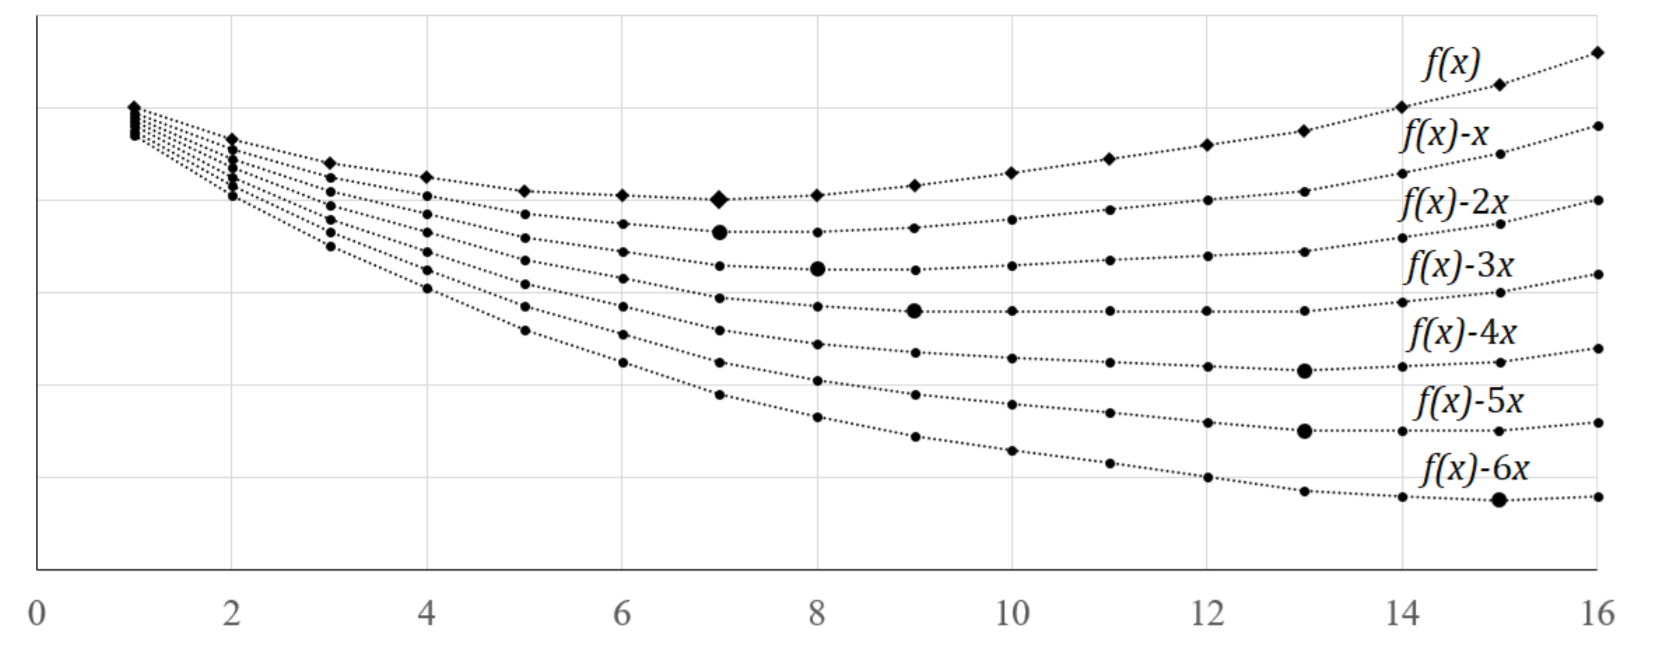
\includegraphics{images/aliensopt}
		\end{center}
		當然,可能會有一個問題出現:就是如果$p$的最小值出現在
	\section{四邊形不等式優化}
	
	所謂四邊形不等式優化,就是俗稱的打表找規律優化。為什麼這樣稱呼呢?因為四邊形不等式優化的滿足條件難以一眼看出  ,有些題目更是難以證明。前國手波路特石曾經說過:「我在選訓二模的時候,看到一題dp,我猜它是四邊形,就用原始的dp式打表找規律,最後AC了。」沒錯,四邊形不等式優化就是那麼玄妙的東西。
	
	\subsection{四邊形不等式與四邊形單調性}
	
	四邊形不等式優化之所以可以對轉移進行加速,是建立在\textbf{四邊形單調性}的基礎上。四邊形單調性是一個雙變數函數的性質,分為凹凸兩種。\\
	
	\definition{四邊形單調性}{
		函數$F$滿足\textbf{凹四邊形單調性},若對於任意的$i<i', j<j'$:\\
		如果$F(j, i) \leq F(j', i)$成立的話,必可以保證$F(j, i') \leq F(j', i')$。\\
		
		函數$F$滿足\textbf{凸四邊形單調性},若對於任意的$i<i', j<j'$:\\
		如果$F(j, i) \geq F(j', i)$成立的話,必可以保證$F(j, i') \geq F(j', i')$。
	}
	
	我們可以把$i$想像成時間,若$i$越大則越接近未來。那麼就可以把凹四邊形單調性想成:若此時(時刻$i$)的$j$比$j'$小,那未來(時刻$i'$)永遠都是$j$比較小。凸四邊形單調也可以用同樣的方式想:若此時$j$比$j'$大,那未來永遠都是$j$比較大。\\
	
	由於當你看到一個函數$F$時,你很難看出這個到底有沒有四邊形單調性,所以我們很常使用\textbf{四邊形不等式}來判斷這個函數的四邊形單調性。\\
	
	\definition{四邊形不等式}{
		\textbf{凹四邊形不等式:}
		
		如果對於任何$ i < i' \leq  j < j'$ 都有 $F(j, i) + F(j', i') \geq F(j, i') + F(j', i)$,則 $F$ 滿足凹四邊
		形單調性。\\
		
		\textbf{凸四邊形不等式:}
		
		如果對於任何$ i < i' \leq  j < j'$ 都有 $F(j, i) + F(j', i') \leq F(j, i') + F(j', i)$,則 $F$ 滿足凸四邊
		形單調性。\\
		
		如果這邊的$i, j$都是整數的話,我們只需要檢查$F(j, i) + F(j + 1, i + 1)$ 和$F(j, i + 1) + F(j + 1, i)$ 的大小關係即可。
	}
	
	滿足四邊形不等式的條件又稱為Monge condition,若一個函數滿足凸四邊形不等式,則必滿足凸四邊形單調性;若一個函數滿足凹四邊形不等式,則必滿足凹四邊形單調性。但是不滿足四邊形不等式的函數不一定沒有四邊形單調性,所以這時候,打表就是你的好幫手了。\\
	
	\problem{四邊形單調性}{
		數學題 - 判斷下列函數是否有凹四邊形單調性:
		\begin{enumerate}
			\item $F(x, y) = xy$
			\item $F(x, y) = (x-y)^2$
			\item $F(x, y) = s_x - t_y$,$s, t$是遞增數列
			\item $F(x, y) = (s_x - s_y)^2$,$s$是遞增數列
			\item $F(x, y) = aA(x, y) + bB(x, y)$,$a, b \geq 0$,$A, B$有凹四邊形單調性
			\item $F(x, y) = (x - y - 1 - K + \sum\limits_{k=x+1}^y C_k)^2$,$C$是正整數數列,$K$是正整數
			\item $F(x, y) = -a_x + a_y - \sqrt{y-x}$,$a$是正整數數列
		\end{enumerate}
	}
	
	\subsection{1D/1D 凸性優化}
	
	這邊要先來個簡單的名詞定義。如果我們說一個dp是$eD/tD$的,代表這個問題有$O(N^e)$個子問題,每個子問題需要$O(N^t)$的時間轉移,所以一個$eD/tD$的dp的總時間複雜度是$O(N^{e+t})$。
	
	\subsubsection{主要思維}
	
	說了這麼多,那四邊形單調性可以幹嘛呢?我們看看以下dp式:
	
	\begin{displaymath}
	dp[i] = \min\limits_{0\leq j < i} \{dp[j] + w(j, i) \}
	\end{displaymath}
	
	這種類型的dp可說是再熟悉不過了,這就是枚舉分段點再加上cost的題型。我們令$F(j, i) = dp[j] + w(j, i)$,如此一來我們在計算每個$dp[i]$時事實上就是在找$F(j, i)$最小的$j$。\\
	
	如果知道$w(j, i)$滿足凸四邊形單調性,那麼$F(i, j)$也會具備凸四邊形單調性,於是就可以套用四邊形不等式優化。\\
	
	1D/1D四邊形不等式凸性優化的精髓在於:如果在某個$i$時,$F(j, i)$比$F(j', i)$大(這裡的$j < j'$),那麼對於所有的時刻$i' > i$永遠都是$F(j, i)$會比較大,所以只要有一時刻從$j'$轉移比從$j$轉移好,就會導致不管未來何時,$j'$一定比$j$好,所以就可以永遠不用從$j$轉移了。\\
	
	\hint{
		我們可以得到一個結論:
		對於所有$i < i'$,$dp[i]$與$dp[i']$的最佳轉移來源$p_i \leq p_{i'}$。(轉移點單調)
	}
	
	我們引述一句蕭電的話:\\
	
	\eeric{
		這與斜率優化的精神很像,就是限制轉移來源。斜率優化用的是斜率單調性,而四邊形則是隨著$i$的遞增,轉移點也會遞增。我們可以用這個遞增的性質來加速轉移過程。
	}
	
	\subsubsection{實作方式}
	
	以下內容會有一些符號約定,這邊先列出來讓讀者更好理解:\\
	\definition{小約定}{
		$i$:時間點,當時間點是$i$就代表你正在計算$dp[i]$的值。\\
		$j$:轉移點,若我說時間點$i$時$j=$某數字就代表$dp[i]$從$j$那裡轉移。\\
		$p$:最佳轉移點,$dp[i]$的最佳轉移點會寫成$p_i$。\\
		$n$:就是$n$,也就是$i$的最大值。
		
		如果出現$i, i', j, j'$,通常表示$i < i'$,而且$j < j'$。
	}
	
	回歸到最原始的dp實作方式,我們在最外層的迴圈跑$i$,而內層迴圈枚舉轉移來源,看看哪個$j$可以使得$F(j ,i)$ 最小,來達到計算每個$dp[i]$的目的。\\
	
	現在套用了四邊形不等式優化,基本計算順序還是不變的,一樣是用一個迴圈跑$i$,逐步把$dp[i]$算出來。不過對於每個$i$都枚舉轉移來源$j$找最好的實在太慢了,就改成用集合維護一些區間,方便以$O(1)$查詢最佳的轉移來源。\\
	
	我們可以把區間$[1, n)$拆成許多不相交的小區間放進集合裡,集合裡的每個元素以$(p, L, R)$的方式儲存。若在時間點$i$時,集合裡面有元素$(p, L, R)$,就代表算到目前為止對於$L\leq i' < R$的$i'$,$dp[i']$的最佳轉移來源就是$p$,也就是說當$i$介於區間$[l, r)$內,則$F(p, i)$就不會比其他$k \not=p$的$F(k, i)$來的大。\\
	那麼我們要怎麼維護這個集合呢?我們考慮以下演算法:
	\begin{enumerate}
		\item 一開始除了$dp[0]$沒有任何$dp[i]$被算出來,所以區間$[1, n)$目前能確定的最佳轉移來源只能是$0$,因此先在集合裡放入區間$(0, 1: n)$。
		\item 當要計算$dp[i]$時,先把右界$R \leq i$的區間從集合中移除(因為這些區間已經不會再被用到了),然後再取右界最小的區間(此區間必包含$i$),從這個區間的$p$處轉移計算$dp[i]$。
		\item 當你計算出了$dp[i]$,那麼之後某些$dp[i']$的最佳轉移來源有可能因此更新成了$i$。這時候因為我們知道$i'$變大時$p_{i'}$只可能不變或變大,所以可以找到一個點$i^*$,使得所有大於等於$i^*$的$i'$的最佳轉移來源統統變成$i$。
		\item 找到這個$i^*$的方法如下:我們考慮右界最大的區間$(p_f, L_f: R_f)$
		\begin{enumerate}
			\item 若$F(i, L_f) \leq F(p_f, L_f)$,則這個區間的最佳轉移來源都即將被$i$取代,所以可以直接將區間拔掉,再考慮右界第二大的區間。
			\item 若$F(i, R_f) \geq F(p_f, R_f)$,恭喜你,什麼事都不用做,因為$p_f$目前還是最好的。
			\item 如果不是上述兩種情況,必然能在這個區間裡找到$i^*$,我們只要二分搜找到$F(i, k) < F(p_f, k)$的最小$k$,就是$i^*$。再從這個$i^*$將區間切成兩段$(p_f, L_f, i^*)$ 與 $(i, i^*: n)$即可。
		\end{enumerate}
	\end{enumerate}
	
	由於這些步驟每次只需要取得右界最大或右界最小的區間,並且放入區間時只會改變到右界最大的區間,所以可以用\inline{deque}來維護這個集合。\\
	
	實作方式與細節如下:(感謝baluteshih)\\
	
	\begin{C++}
		struct seg{int p,l,r;};
		deque<seg> deq;
		void solve(){
			deq.push_back(seg{0,1,n});
			for(int i=1; i<n; i++){
				// 計算dp[i]
				while(deq.front().r <= i) deq.pop_front();
				dp[i] = f(deq.front().p, i);
				// 更新以 i 作為轉移來源的區間
				while(deq.size() &&
				f(i, deq.back().l) < f(deq.back().p, deq.back().l))
				deq.pop_back();
				seg new_seg = seg{i, i+1, n};
				if(deq.size()){ // 有可能全部被 pop 掉
					int c = binary_search(deq.back().p, i);
					// c 是滿足 f(i, k) < f(deq.back().i, k) 的最小 k
					deq.back().r = new_seg.l = c;
				}
				if(new_seg.l < n) deq.push_back(new_seg);
			}
		}
	\end{C++}
	
	當然,你要先確定你的函數$F$有凸四邊形單調性。
	
	\subsection{1D/1D 凹性優化}
	
	凹性優化的題目十分罕見,不過還是有凹性優化的實作方式。\\
	
	與凸性優化的概念一樣,只不過相較於凸單調性,凹單調性可以推知:對於所有$i < i'$,$dp[i]$與$dp[i']$的最佳轉移來源$p_i \geq p_{i'}$。\\
	
	所以我們可以把凸性優化的\inline{deque}改成用\inline{stack}維護由上到下是$p$遞減(也就是區間遞增),每次插入一個新區間的時候因為裡面的所有$p$都比較小,所以會先動到(可能pop)數字大的。故top處放右界最小的區間,計算$dp$值時從top處pop掉不會再被用到的區間,然後選擇右界最小的區間轉移,每算完一個$dp[i]$,一樣從top處慢慢pop,再用二分搜找到$i^*$,不過因為是凸單調性,所以這裡的區間要拆成$(i+1, i^*)$與$(i^*, L_f)$兩部分。\\
	
	實作細節與凸性優化差不多,這邊就不列code了。
	
	\subsection{2D/1D 凸性優化}
	
	2D/1D 就是狀態二維,但轉移只有一維的dp,一般來說會長這樣:
	
	\begin{displaymath}
	dp[i][j] = \min\limits_{i\leq k < j} \{ dp[i][k] + dp[k][j] + w(i, j) \}
	\end{displaymath}
	
	這邊與1D/1D一樣,假設$w(i, j)$符合凸四邊形單調性,那麼通常$dp[i][j]$就滿足凸四邊形單調性。所以這邊可以枚舉$i$,讓dp狀態變成一維,就可以用$N$次的1D/1D解決,時間複雜度$O(N^2\log N)$。\\
	
	\hint{如果 $w(i, j)$ 為凸單調性的且 $w(i, i + 2) \geq \max(w(i, i + 1), w(i + 1, i + 2))$,則 $dp[i][j]$ 也會符合凸單調性}
	
	2D/1D凸性優化還有一個神奇的性質,不僅可以增加效率、降低時間複雜度,還可以大大的減低實作難度。\\
	
	這邊要介紹一個定理:\\
	
	\theorem{2D/1D 凸性優化}{
		設 $p_{i,j}$ 是 $dp[i][j]$ 在轉移時所找到的最佳轉移點,且 $dp$ 滿足凸四邊形不等式,則:
		\begin{displaymath}
		p_{i, j − 1} \leq p_{i, j} \leq p_{i + 1, j}
		\end{displaymath}
	}
	
	神奇的證明如下:先假設$p_{i, j-1} = k_1$,$p_{i, j} = u$,$p_{i+1, j} = k_2$,我們使用反證法,分兩邊討論:
	
	\begin{enumerate}
		\item 假設$k_1 > u$,則 $u+1 < k_1+1 \leq j-1 < j $,根據四邊形不等式可以得到:
		\begin{displaymath}
		dp[u+1][j-1] + dp[k_1+1][j] \leq dp[u+1][j] + dp[k_1+1][j-1]
		\end{displaymath}
		再利用$u$是$dp[i][j]$的最佳轉移來源的性質,可以列出以下式子:
		\begin{displaymath}
		dp[i][u] + dp[u+1][j] \leq dp[i][k_1] + dp[k_1+1][j]
		\end{displaymath}
		將以上兩不等式相加,可得:
		\begin{displaymath}
		dp[i][u] + dp[u+1][j-1] \leq dp[i][k_1] + dp[k_1+1][j-1]
		\end{displaymath}
		但這樣一來$k_1$就不是$p_{i, j-1}$了(因為選$u$的話更好),所以$k_1 \leq u$。
		
		\item 再假設$u > k_2$,可以用同樣方法,利用 $i < i+1 \leq k_2 < u $,列出四邊形不等式,再用$k_2$是$dp[i+1][j]$的最佳轉移來源,列出$dp$從$k_2$轉移與從$u$轉移的比較,最後再將兩不等式相加,就可以推出$u \neq p_{i, j}$的矛盾,因此$u \leq k_2$。
	\end{enumerate}
	
	如此一來我們得到了$k_1 \leq u \leq k_2$,定理得證。
	
	\subsubsection{實作}
	
	根據上述定理,我們可以發現到:$dp[i][j]$ 的轉移來源可以從區間 $[p_{i,j−1}, p_{i+1,j} ]$ 這個區間內找到,如果我們先計算$i-j$較小的$dp[i][j]$,並且記錄最佳的轉移點的話,枚舉範圍縮小了,就可以減少許多枚舉時間。\\
	
	那麼總共會省多少時間呢?我們可以考慮計算完一個 dp 表格的斜排 (也就是 $j - i$ 固定) 所需的時間:
	
	\begin{displaymath}
	\vdots
	\end{displaymath}
	\begin{displaymath}
	p_{i−2,j−3} \leq p_{i−2,j−2} \leq p_{i−1,j−2}
	\end{displaymath}
	\begin{displaymath}
	p_{i−1,j−2} \leq p_{i−1,j−1} \leq p_{i,j−1}
	\end{displaymath}
	\begin{displaymath}
	p_{i,j−1} \leq p_{i,j} \leq p_{i+1,j}
	\end{displaymath}
	\begin{displaymath}
	p_{i+1,j} \leq p_{i+1,j+1} \leq p_{i+2,j+1}
	\end{displaymath}
	\begin{displaymath}
	p_{i+2,j+1} \leq p_{i+2,j+2} \leq p_{i+3,j+2}
	\end{displaymath}
	\begin{displaymath}
	\vdots
	\end{displaymath}
	
	看出來了嗎?中間那行是同一個斜排的不同$dp[i][j]$的轉移來源,這些轉移來源的區間正好是連續的並且這些轉移來源會隨著$i$遞增而遞增,所以計算一個斜排所需的時間僅僅是$O(N)$!一個狀態2D的dp表格頂多$O(N)$個斜排,所以總時間複雜度$O(N^2)$!\\
	
	這邊是2D/1D凸性優化的核心代碼:\\
	
	\begin{C++}
		for(int len = 2; len <= n; len++){  // 枚舉區間長度 (i - j)
			for(int i = 1, r = len; j <= n; i++, j++){
				// 枚舉長度為 len 的所有區間
				dp[i][j] = INF;
				for (int k = p[i][j-1]; k <= p[i+1][j]; k++)
				if (dp[i][j] > dp[i][k] + dp[k+1][j] + w(i, j)){
					// 更新 dp 陣列
					dp[i][j] = dp[i][k] + dp[k+1][j] + w(i, j);
					p[i][j] = k;  // 記錄(最小)轉移來源
				}
			}
		}
	\end{C++}
	
	\subsection{2D/1D 凹性優化}
	
	凹性沒有好性質 QQ\\
	
	所以只能枚舉$i$,讓dp狀態變成一維,用$N$次的1D/1D解決了。時間複雜度$O(N^2\log N)$。
	
	\subsection{習題}
	\problem{超大畫框設置(TIOJ 1283)}{
		給定一個類似這樣的多邊形:(線皆垂直,且上面為右下右下⋯⋯,下面為下右下右下右⋯⋯),請問裡面可以放的最大矩形面積為何?(總邊數$\leq 10^5$)
		\begin{center}
			%\includegraphics[width=0.5\textwidth]{images/1283_1}
		\end{center}
		
	}
	\problem{AI-666 賺多少(TIOJ 2039)}{
		你想要在股市賺錢:總共有$T$天,每天股市都有一個價格為$V_i$,你可以做買入或賣出,但是有一些限制:
		\begin{itemize}
			\item 只能先買後賣,不可以先賣後買。
			\item 每次買與賣都限定是一個單位的商品。同時,在買入之後,賣出之前,不可以再買入。
			\item 由於法令的規定,在此期間內最多只能進行$K$次的交易(一次交易包含買賣各一次)。
		\end{itemize}
		給定$T, V_i, K$,請問能得到的最大獲益為何?($K \leq N \leq 2 \times 10^6, V_i \leq 10^7$)
	}
		
			